\section{extract}
\index{extract}
\label{sec:extract}

It extracts simulation information. It does not write information on screen, but returns it as a variable. If you want to see something on screen, use the \param{lowmsg} command to print it.

\begin{description}

\item [ac.coverage]\index{ac.coverage} Returns the surface hydrogen coverage in epitaxial models, as a $[0-1]$ value (ML or monolayer).

\item [ac.max]\index{ac.max} Returns a list with the maximum values for the Lattice KMC interface position in x, y and z. Accepts the optional arguments  \param{min.x=$<$minx$>$}, \param{max.x=$<$max.x$>$}, \param{min.y=$<$miny$>$}, \param{max.y=$<$max.y$>$},  \param{min.z=$<$minz$>$} and \param{max.z=$<$max.z$>$} to limit the extraction domain size. 

\item [ac.mean]\index{ac.mean} Returns a list of the mean value of the Lattice KMC interface position in x, y and z respectively. Accepts the optional arguments  \param{min.x=$<$minx$>$}, \param{max.x=$<$max.x$>$}, \param{min.y=$<$miny$>$}, \param{max.y=$<$max.y$>$},  \param{min.z=$<$minz$>$} and \param{max.z=$<$max.z$>$} to limit the extraction domain size. 

\item [ac.min]\index{ac.min} Returns a list with the minimum values for the Lattice KMC interface position in x, y and z. Accepts the optional arguments  \param{min.x=$<$minx$>$}, \param{max.x=$<$max.x$>$}, \param{min.y=$<$miny$>$}, \param{max.y=$<$max.y$>$},  \param{min.z=$<$minz$>$} and \param{max.z=$<$max.z$>$} to limit the extraction domain size. 

\item [ac.stdev]\index{ac.stdev} Returns a list of the standard deviation of the Lattice KMC interface in x, y and z respectively. Accepts the optional arguments  \param{min.x=$<$minx$>$}, \param{max.x=$<$max.x$>$}, \param{min.y=$<$miny$>$}, \param{max.y=$<$max.y$>$},  \param{min.z=$<$minz$>$} and \param{max.z=$<$max.z$>$} to limit the extraction domain size. 

\item [amorphous.fraction]\index{amorphous.fraction} Returns the fraction of space that is amorphous in an {\tt OKMC} enviroment for the material specified in the required option \param{material=$<$mt$>$}. For more information, read Section \ref{sec:amorph}.

\item [configuration]\index{configuration} Comparing \MMonCa\ effective configurations is not always straightforward, especially when parameters were overruled in the simulation script. This command enables one to dump all the actual configuration to the log or a file. All dump invocations must be preceded by the init command. Any configuration parameter overruled after this command does not affect the already happened dump content. If the optional argument \param{filename} is given, the configuration is dumped into the given file; otherwise into a Tcl variable. The format is \param{key:data type:value}.

\item [coord=$<$x y z$>$]\index{coord} Uses the coordinate x, y and z as the starting center to look for neighbors in the \param{coordination} command.

\item [coordination]\index{coordination} Returns a list of neighbors, distance to it, the neighbor type and total account of neighbor types. It requires the use of the option \param{coord} to specify the value of the coordinate to use as a center and \param{radius} for the look-up radius. It buils a crystal as a sphere with the specified radius plus 0.5 nanometers, so the specified coordinate should be close to 0 0 0.

\item [count.defects]\index{count.defects} Returns how many defects are in the simulation. It accepts the following options to ``filter'' the results: \param{material} for a particular material, \param{name} to specify a particle name, \param{defect} for a defect name, \param{min.size} for a minimum size and \param{ID} for a particular defect type.

\item [count.particles]\index{count.particles} Returns how many particles are in the simulation. It accepts the following options to ``filter'' the results: \param{material} for a particular material, \param{particle} to specify a particle name, \param{defect} for a defect name, \param{min.size} for sizes equal or bigger and \param{ID} for a particular defect type. It is different from \param{count.defects}. For instance, a B2I3 cluster will return 3 interstitial particles, but only 1 defect.

\item [count.positions]\index{count.positions} Returns how many particles are in a particular position. It requires the argument \param{position}\index{position} and accepts the argument \param{material} to filter the particles to the specified material. 

\item [defect]\index{defect} Parameter used by \param{histogram} to specify the defect type. Also used by \param{profile} to restrict the output to a particular cluster.

\item [defect.radius]\index{defect.radius} It computes the average radius (in nm) of the specified defects. It requires the parameter \param{defect} and accepts the optional parameters \param{ID} to specify a particular type and \param{min.radius} to set up a threshold that defines when a defect is ``visible'' and will be included in the calculation.

\item [defects=$<$list$>$]\index{defects} Returns all the defects (OKMC particles) and positions in the simulation. If all the defects are requested, an empty list (defects=\{ \}) is to be provided. Otherwise, an enumeration of the defects requested, separated by spaces, is to be provided. For MobileParticles, \param{MobileParticle} has to be specified. For other defects, the defect name (eg. \param{ICluster}, \param{VCluster}) is to be written. If alloy atoms are requested, type \param{Alloy}.

\item [diffusivity]\index{diffusivity} Returns the diffusivity of the specified particle \param{name} in the specified  \param{material}. It does not work for I or V particles. If \param{macroscopic} is specified, then it tracks the diffusivity of the whole family of particles associated. Use \param{extract reset} to start measuring.

\item [dimension]\index{dimension} Sets the dimension to collapse the output. Accepts 0, 1 2 and 3. If 0 is specified, no geometrical information is obtained, just a value with the overall mean value.

\item [dose]\index{dose} Extracts the damage recieved by the material by the \param{cascade} command. The units are in dpa. This command assumes that the cascades contain Frenkel pairs, that is, same number of interstitials and vacancies (accepts clusters but the total ammount of interstitials and vacancies must remain equal), if not this command will give an underestimated or overestimated dpa value.

\item [histogram]\index{histogram} Requires the parameters \param{defect} and \param{material}. Returns a histogram for the given defect/s name. Several defects can be used separated by commas, for instance {\tt ICluster,VCluster}. A histogram is considered a list of cluster names and the number of them present when issuing the command. 

\item [file=$<$filename$>$]\index{file} This option can be added to {\em any} of the previous parameters to write the results in filename.

\item [fuzz]\index{fuzz} Returns a ``y z depth'' array listing all the depths at which a free interface was detected.

\item [jumps]\index{jumps} Returns the number of jumps for the mobile particle specified in the required option \param{name=$<$pt$>$}

\item [material.location]\index{material.location} Returns the long material name at the location given by \param{x=$<$value$>$}, \param{y=$<$value$>$} and \param{z=$<$value$>$}. It can be used to unit test material definition Tcl functions or JSON files.

\item [material.map]\index{material.map} Extracts the internal mesh's material attributes. For the sake of simple implementation, it represents each mesh cell with a slightly smaller cell, with each corner having the material attribute of the cell. This file is best viewed using linear interpolation, for example in Paraview. The linear interpolation of the thin layers between the cells are to be ignored. The material attributes in the VTK file come from the internal MMonCa representation, which is also visible in the log. Requires the \param{filename=$<$VTK filename$>$}

\item [min.radius]\index{min.radius} Optional parameter for \param{defect.radius}. It considers only ``visible'' defects with radius equal or bigger than the specified one.

\item [min.size]\index{min.size} Optional parameter for \param{count.defects} or \param{count.particles}. It limits the count to defects with size equals or bigger than the specified. The size of a defect is defined as its total number of particles.

\item [profile]\index{profile} Returns the concentration for the particle specified in the required option \param{name=$<$pt$>$}. When simulating binary alloys it is possible to extract the atom counters of the A and B species in the AB binary alloy with the \param{name=A.atoms} and \param{name=B.atoms} respectively. Also it is possible to extract the profile of the A atoms of the AB binary alloy by no introducing the \param{name} keyword and introducing the desired material profile with the \param{material} keyword. LKMC information can also be extracted through \param{name=lkmc.defects} and \param{name=lkmc.ac} options and corresponding to defective configurations and amorphous/crystalline interface respectively. Additonal OKMC options are in the examples.

\item [profile.damage]\index{profile.damage} Returns the damage concentration (i.e. self-Interstitials and Vacancies) for the material specified in the required option \param{material=$<$mt$>$}. Such concentration saturates at the {\tt amorphization.threshold} value. For more information, read Section \ref{sec:amorph}.

\item [profile.mobile]\index{profile.mobile}  Returns the mobile concentration for the mobile particle specified in the required option \param{name=$<$pt$>$}. It assumes $[X] = \mathrm{jumps} / (\Delta t \Delta V \nu(pt))$.

\item [reset]\index{reset} Resets the information for mobile particles. It allows incremental displays of properties for mobile particles. If \param{reset} is not used, then all the properties for mobile particles are accounted from the very beggining of the simulation, otherwise, the magnitudes are an average between the last reset and the current time.

\item [strain.xy] Returns the shear strain (xy) loaded into OKMC in a 2D X/Y projection.

\item [time]\index{time} Returns the current simulated time.

\end{description}

\subsection{Examples}
\begin{itemize}
\item \verb+extract count.particles defect=ICluster+ Extracts how many particles are in "ICluster"
\item \verb+extract count.particles defect=VCluster ID=V3+ Extracts how many particles are contained in V3 in "VCluster".
\item \verb+extract diffusivity macroscopic name=He material=Copper+
\item \verb+extract time+
\item \verb+extract ac.mean+ Extracts a list containing the x, y and z mean values of amorphous/crystalline interface positions. Use \verb+[lindex [extract ac.mean] 0]+ to extract the x mean value.
\item \verb+extract histogram defect=<111> material=Iron+ 
\item \verb+extract profile name=Cr dimension=1 material=Iron+ Extracts the profile [$cm^{-3}$] of the Cr atoms collapsed to the X-dimension
\item \verb+extract profile material=Iron+ Extracts the profile [$cm^{-3}$] of the Iron lattice atoms (computed from the cell counters)
\item \verb+extract profile name=X*+ Extracts the profile for all the active (not clustered) X atoms.
\item \verb+extract profile defect=* name=X+ Extracts the profile for all clustered B atoms such that a \ch{B3} cluster is counted three times.
\item \verb+extract profile defect=BICs material=Silicon name=B2I+ Extracts the profile for the \ch{B2I} cluster within the BICs family.
\item \verb+extract profile defect=BICs material=Silicon name=B*+ Extracts the profile for all clustered B atoms within the BICs cluster family, such that a \ch{B3} cluster is counted three times.
\item \verb+extract profile defect=BICs material=Silicon+ Extracts the profile for all BICs clusters.
\item \verb+extract material.map filename="materials.vtk"+ Extracts the VTK file rendered in Fig.\ref{fig-vtk-export-cut} from the JSON mesh description below.
\end{itemize}

\begin{figure}[!htb]
  \centering
  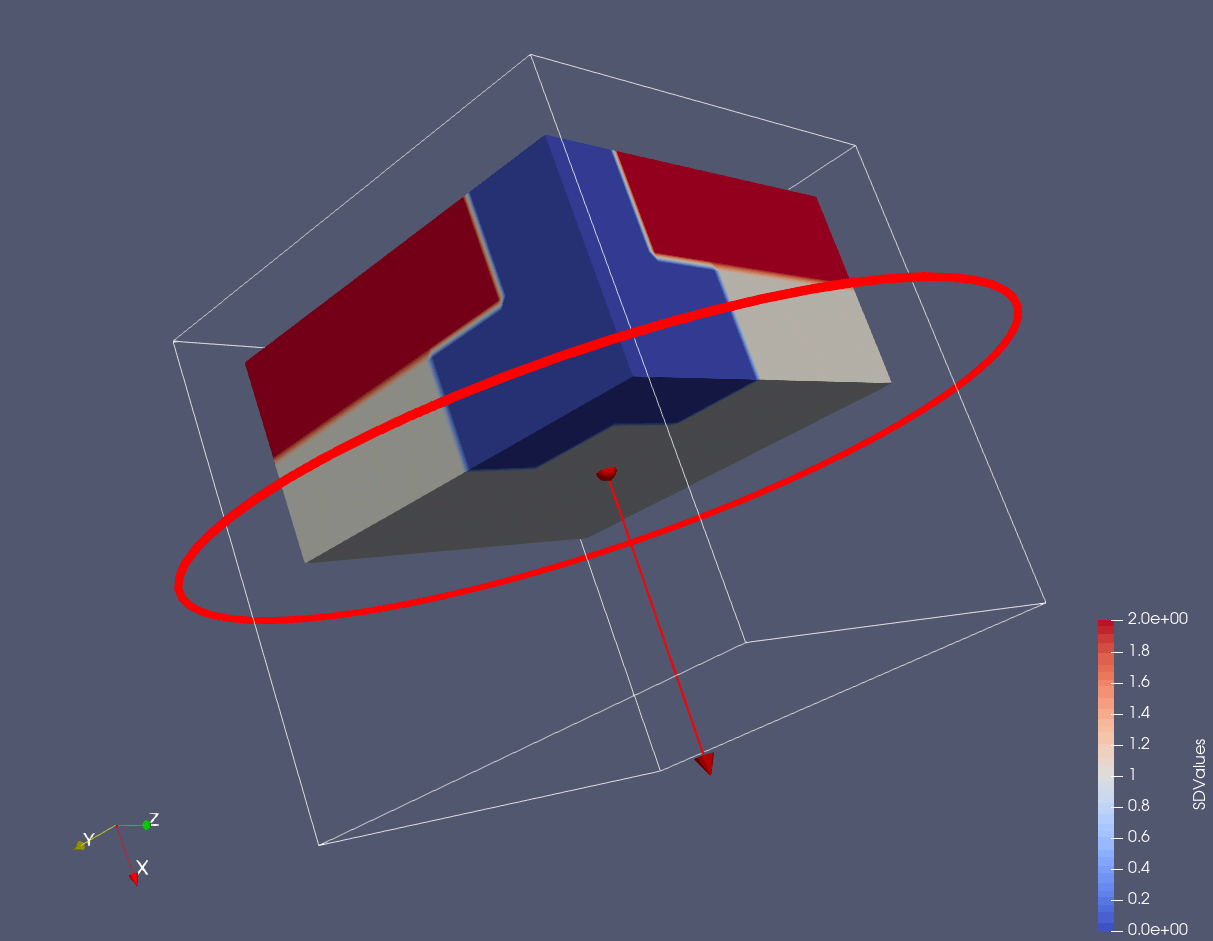
\includegraphics[width=1.0\textwidth]{images/vtk-export-cut.png}
  \caption{\label{fig-vtk-export-cut} Clipped rendering of the VTK file exported from the JSON mesh below}
\end{figure}

\begin{lstlisting}
{
  "linesX": [
    0.0, 1.5, 3.0, 4.5, 6.0
  ],
  "linesY": [
    0.0, 1.4, 2.8, 4.4, 6.0
  ],
  "linesZ": [
    0.0, 1.3, 2.6, 3.9, 6.0
  ],
  "materialIDs": [
    0, 2, 2, 2, 2, 2, 2, 2, 2, 2, 2, 2, 2, 2, 2, 2,
    0, 0, 1, 1, 0, 1, 1, 1, 1, 1, 1, 1, 1, 1, 1, 1,
    0, 0, 1, 1, 0, 1, 1, 1, 1, 1, 1, 1, 1, 1, 1, 1,
    0, 1, 1, 1, 1, 1, 1, 1, 1, 1, 1, 1, 1, 1, 1, 1
  ],
  "materialMapping": {
    "SiO2": 0,
    "Silicon": 1,
    "SiliconGermanium": 2
  }
}
\end{lstlisting}
